\section{Aufbau}
\begin{figure}
	\centering
	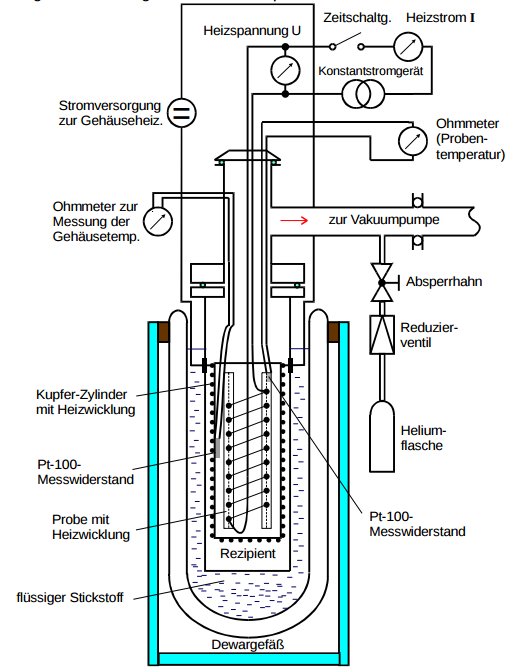
\includegraphics[width=0.6\textwidth,]{graphics/aufbau.png}
	\caption{Skizzenhafter Aufbau des Versuchs. \cite{skript}}
	\label{fig:aufbau}
\end{figure}
Der Versuchsaufbau ist in \ref{fig:aufbau} dargestellt.
In einem \emph{Dewargefäß} befindet sich der \emph{Rezipient} und im Rezipienten befindet sich die \emph{Probe mit Heizwicklung}, das von einem \emph{Kupfer-Zylinder mit Heizwicklung} umgeben ist.
Die Heizwicklungen der Probe und des Kupferzylinders arbeiten unabhängig voneinander.
Der Rezipient ist mit Gas befüllbar und kann mittels einer Vakuumpumpe evakuiert werden. 
Die Temperaturmessung von Probe und Kupferzylinder wird durch zwei \emph{Pt-100-Messwiderständen}, je eine an beiden Heizungen, ermöglicht.


\section{Durchführung}
\label{sec:durchfuehrung}
Es wird die Temperatur-Abhängigkeit der Molwärme $C_p$ von Kupfer im
Bereich von $\SI{80}{\kelvin}$ bis $\SI{300}{\kelvin}$ gemessen.
Zum Kühlen der Probe wird der Rezipient mit gasförmigen Helium geflutet
und das Dewar-Gefäß mit flüssigem Stickstoff gefüllt.
Auf diese Weise stellt sich ein Temperaturgleichgewicht zwischen Probe und Stickstoff ein und die Probe wird auf die Temperatur flüssigen Stickstoffs $T=\SI{90}{\kelvin}$ \cite{stickstoff} gekühlt.
Nach Abkühlen der Probe wird der Rezipient evakuiert.
Weiter sollen während des Versuches die Temperatur der Probe und die Temperatur des die Probe umhüllenden Kupferzylinders möglichst gleich sein.
Dies wird erforderlich, um Störeffekte durch Wärmestrahlung und Konvektion auszuschließen und die Energiebilanz der Kupferprobe auf die reine Wärme-Aufnahme zu beschränken. 
Über die Probenheizung kann der Probe Wärme zugeführt werden, 
während die davon unabhängige Heizung die Gehäusetemperatur auf Probentemperatur hält.
Es wird die Probenheizspannung $U$, Probenheizstrom $I$ und die Zeit $t$ in Abschnitten notiert, 
in welchen die Probe um $\SI{7}{\kelvin}$ bis $\SI{11}{\kelvin}$ erwärmt wird.
